\documentclass{article}
\usepackage[utf8]{inputenc}
\usepackage{graphicx} % takes care of graphic including machinery
\usepackage{cmbright} % Change font
\usepackage[OT1]{fontenc}
\usepackage[super]{nth}

%%%%%%%%%%%%%%%%%%%%%%%%%%%%%%%%%%%%%%%%%%%%%%%%%%%%%%%%%%%%%%%%%%%%%%%%%%
%%%%%%%%%%%%%%%%%%%%%%%%%%%%%%%%%%%%%%%%%%%%%%%%%%%%%%%%%%%%%%%%%%%%%%%%%%
\title{A Measurement of the Compton Wavelength}
\author{Springer PHYS 3719-001 Spring 2021, Pierce Jorgensen}
\date{\today}

\begin{document}

\maketitle

%%%%%%%%%%%%%%%%%%%%%%%%%%%%%%%%%%%%%%%%%%%%%%%%%%%%%%%%%%%%%%%%%%%%%%%%%%
%%%%%%%%%%%%%%%%%%%%%%%%%%%%%%%%%%%%%%%%%%%%%%%%%%%%%%%%%%%%%%%%%%%%%%%%%%
\section{Abstract}

An experiment to demonstrate the credibility of quantum mechanics and special relativity by means of examining the Compton Effect. Using a Caesium source and an Aluminum target we can observe the effects of Compton Scattering by measuring the angle and peak energies of recoil photons. From these measurements we determined the Compton Wavelength; a ratio between Planck's constant, electron mass, and the speed of light. These findings establish a relationship between special relativity and quantum theory, and show that the nature of light cannot be explained as a purely wave-like phenomenon; thus demonstrating the validity of these two fields of study.

%%%%%%%%%%%%%%%%%%%%%%%%%%%%%%%%%%%%%%%%%%%%%%%%%%%%%%%%%%%%%%%%%%%%%%%%%%
%%%%%%%%%%%%%%%%%%%%%%%%%%%%%%%%%%%%%%%%%%%%%%%%%%%%%%%%%%%%%%%%%%%%%%%%%%
\section{Introduction}

In the early \nth{20} century, research into matter and X-ray behavior was ongoing. An experiment was designed to measure the deflection of X-Ray photons against a carbon target, and it was discovered that the deflected rays exhibited a shift in wavelength that increased with a greater scattering angle. It wasn't until 1923 when Arthur Holly Compton was able to explain this phenomena. He proposed a particle model for the photon and applied the laws of conservation of energy and momentum. Surprisingly, the results were consistent with how particles behave in collision experiments, and thus Compton concluded that photons cannot be described as having a wave-like nature alone. Light behaves as a stream of particles with an energy proportional to the wavelength. \cite{Compton} \par

In his paper published in the Physical Review \cite{Phys_Review}, Compton described this using an equation involving the scattering angle, and wavelengths before and after collision.
\begin{equation}
    \lambda' - \lambda = \frac{h}{m_{e}c}(1-cos\theta)
\end{equation}
This relationship demonstrates not only that photons undergo collisions, but that these results can only be predicted by using constants that are derived from quantum theory. Thus it validates the proposals made by quantum mechanics and provides much deeper insight into the nature of photons.

%%%%%%%%%%%%%%%%%%%%%%%%%%%%%%%%%%%%%%%%%%%%%%%%%%%%%%%%%%%%%%%%%%%%%%%%%%
%%%%%%%%%%%%%%%%%%%%%%%%%%%%%%%%%%%%%%%%%%%%%%%%%%%%%%%%%%%%%%%%%%%%%%%%%%
\subsection{Purpose}

In this experiment we will attempt to obtain the aforementioned ratio using the equation for Compton Wavelength. By doing so we will provide further evidence to support the theory, as well as gain experience in proper statistical measurement and data analysis.

%%%%%%%%%%%%%%%%%%%%%%%%%%%%%%%%%%%%%%%%%%%%%%%%%%%%%%%%%%%%%%%%%%%%%%%%%%
%%%%%%%%%%%%%%%%%%%%%%%%%%%%%%%%%%%%%%%%%%%%%%%%%%%%%%%%%%%%%%%%%%%%%%%%%%
\subsection{Hypothesis}

We predict that by measuring the difference in wavelength between incident photons and photons deflected by an angle theta, we can determine the ratio between Planck's constant, electron mass, and the speed of light.

%%%%%%%%%%%%%%%%%%%%%%%%%%%%%%%%%%%%%%%%%%%%%%%%%%%%%%%%%%%%%%%%%%%%%%%%%%
%%%%%%%%%%%%%%%%%%%%%%%%%%%%%%%%%%%%%%%%%%%%%%%%%%%%%%%%%%%%%%%%%%%%%%%%%%
\section{Methods}

In this experiment we used a Caesium-137 source and a Cobalt-60 source for calibration. 
First the Caesium source is stored in an enclosure of lead bricks, with a small opening point that can be obscured when not taking measurements. 
A 200 Volt power supply is then connected to a photo-multiplier tube, with a Sodium Iodide crystal scintillator. 
This creates a shower of lower energy photons which go through 10 multipliers. Then the tube is connected to two amplifiers that together create an output of 10 microsecond pulses. 
The signal is sent to a multichannel analyzer so that the pulse heights can be recorded in bins on a histogram. 
To record output, Maestro data analysis software was used. \par

After the equipment is set up, first a $^{60}$Co source or other known source is used to calibrate the measurements. $^{60}$Co has two known peaks of $1.1732$ MeV and $1.3325$ MeV. When that's done, place the detector directly in front of the $^{137}$Cs source and remove the blocking material to start taking measurements. This incident angle should give a peak energy of about $662$ keV for a typical source, which will be considered wavelength $\lambda$. Then place an Aluminum rod in front of the source so that the beam will encounter the material and be deflected. Place lead bricks at angles where the beam is not being measured to reduce the amount of stray photons. Then place the detector at different angles from the incident of the beam, pointing the face of the detector directly at the Aluminum rod. Peak energies taken at these deflection angles are considered wavelength $\lambda'$. 

%%%%%%%%%%%%%%%%%%%%%%%%%%%%%%%%%%%%%%%%%%%%%%%%%%%%%%%%%%%%%%%%%%%%%%%%%%
%%%%%%%%%%%%%%%%%%%%%%%%%%%%%%%%%%%%%%%%%%%%%%%%%%%%%%%%%%%%%%%%%%%%%%%%%%
\section{Results}

The $^{137}$Cs source used was shown to have an average peak energy at incident angle $\theta_{0}$ of $650.199 \pm 0.083$ keV. From this we can infer that our measurements at incident angle are not within one sigma of the expected value of $662$ keV. Therefore, we will use the known value for peak energy of $^{137}$Cs to calculate incident wavelength $\lambda$.

%%%%%%%%%%%%%%%%%%%%%%%%%%%%%%%%%%%%%%%%%%%%%%%%%%%%%%%%%%%%%%%%%%%%%%%%%
\begin{center}
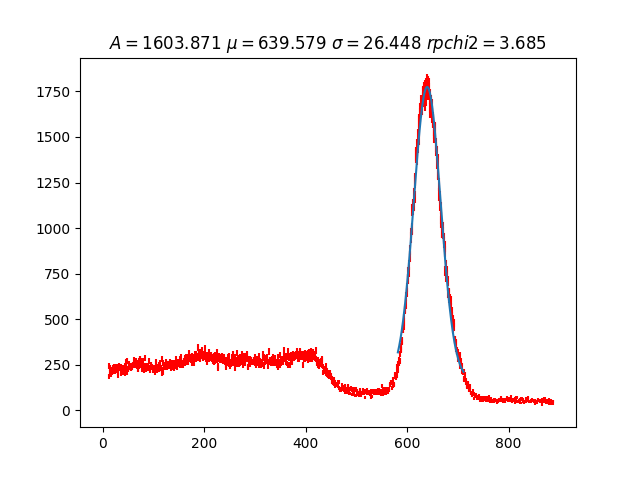
\includegraphics[scale=0.65]{Data/Wavelength_Data/compton_fit_thet_0_fit.png} \\
\caption[1]{ Peak energy distribution of radiation deflected at incident angle $\theta=0^{\circ}$. The horizontal axis is the energy in keV, and the vertical axis is bin height. A is the maximum bin height, $\mu$ is the best estimate for peak energy, $\sigma$ is the standard deviation, and $rpchi2$ is the estimate on reduced chi-squared $\widetilde\chi^{2}$.}
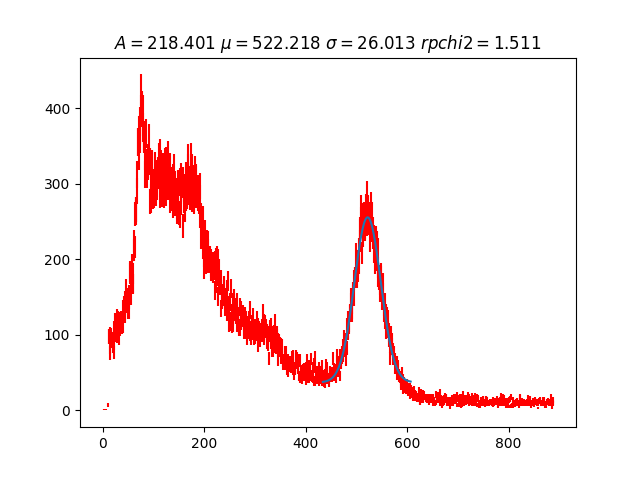
\includegraphics[scale=0.65]{Data/Wavelength_Data/compton_fit_thet_30_fit.png} \\
\caption[2]{ Energy distribution of radiation deflected at $\theta=30^{\circ}$}
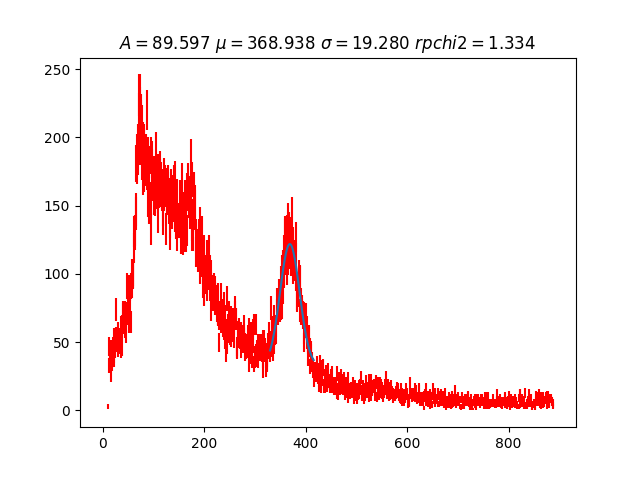
\includegraphics[scale=0.65]{Data/Wavelength_Data/compton_fit_thet_60_fit.png} \\
\caption[3]{ Energy distribution of radiation deflected at $\theta=60^{\circ}$}
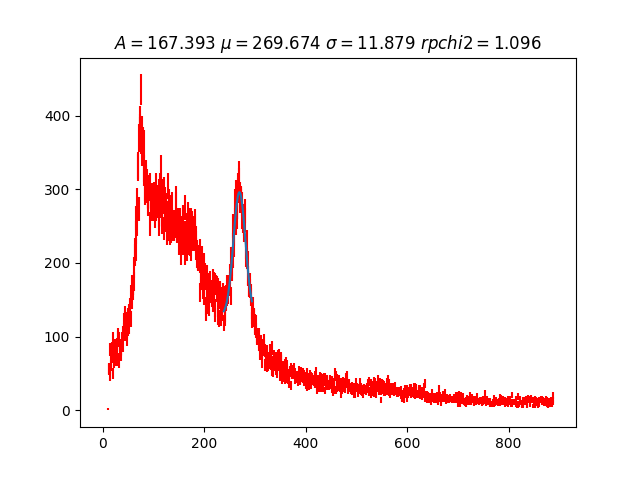
\includegraphics[scale=0.65]{Data/Wavelength_Data/compton_fit_thet_90_fit.png} \\
\caption[4]{ Energy distribution of radiation deflected at $\theta=90^{\circ}$}
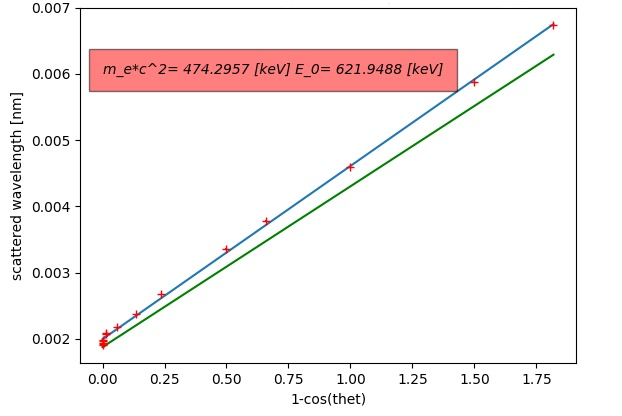
\includegraphics[scale=0.6]{Data/Analysis/lambda_vs_cos_angle.jpg} \\
\caption[5]{ Wavelength measured in nanometers as a function of theta. $\lambda$ vs $1-cos(\theta)$} \vspace{5mm}

%%%%%%%%%%%%%%%%%%%%%%%%%%%%%%%%%%%%%%%%%%%%%%%%%%%%%%%%%%%%%%%%%%%%%%%%%%
\begin{tabular}{| c | c | c | c | c | c |}
    \hline
     Theta (degrees) & $\mu \pm \sigma_{\mu}$ [keV] & $\widetilde\chi^{2}$ & $\lambda$ [pm] & $h$/$m_{e}c$ \\
     \hline
     -10 & $597.662 \pm 0.113$ & 1.233 & $2.075 \pm 0.024$ & $13.63 \pm 8.131 \cdot 10^{-12}$ \\
     \hline
     -5 & $631.620 \pm 0.096$ & 3.184 & $1.963 \pm 0.019$ &  \\
     \hline
     -1 & $650.199 \pm 0.083$ & 5.506 & $1.907 \pm 0.016$ &  \\
     \hline
     0 & $639.579 \pm 0.083$ & 3.685 & $1.939 \pm 0.016$ &  \\
     \hline
     1 & $646.856 \pm 0.056$ & 5.273 & $1.917 \pm 0.011$ &  \\
     \hline
     5 & $625.191 \pm 0.073$ & 4.578 & $1.983 \pm 0.014$ &  \\
     \hline
     10 & $594.347 \pm 0.138$ & 1.315 & $2.086 \pm 0.029$ & $14.02 \pm 9.734 \cdot 10^{-12}$ \\
     \hline
     20 & $568.525 \pm 0.264$ & 1.003 & $2.181 \pm 0.058$ & $5.091 \pm 4.793 \cdot 10^{-12}$ \\
     \hline
     30 & $522.218 \pm 0.237$ & 1.511 & $2.374 \pm 0.056$ & $3.740 \pm 2.085 \cdot 10^{-12}$ \\
     \hline
     40 & $464.383 \pm 0.319$ & 1.153 & $2.670 \pm 0.085$ & $3.407 \pm 1.780 \cdot 10^{-12}$ \\
     \hline
     60 & $368.938 \pm 0.304$ & 1.334 & $3.361 \pm 0.102$ & $2.976 \pm 1.001 \cdot 10^{-12}$ \\
     \hline
     70 & $327.725 \pm 0.448$ & 0.795 & $3.783 \pm 0.169$ & $2.903 \pm 1.261 \cdot 10^{-12}$ \\
     \hline
     90 & $269.674 \pm 0.185$ & 1.096 & $4.598 \pm 0.085$ & $2.725 \pm 0.421 \cdot 10^{-12}$ \\
     \hline
     120 & $211.072 \pm 0.215$ & 0.877 & $5.874 \pm 0.126$ & $2.667 \pm 0.413 \cdot 10^{-12}$ \\
     \hline
     145 & $183.921 \pm 0.137$ & 1.276 & $6.742 \pm 0.092$ & $2.677 \pm 0.250 \cdot 10^{-12}$ \\
     \hline
     
\end{tabular} \\ \vspace{4mm}
\caption[6]{ Results of Compton Scattering experiment. Calculation of $h$/$m_{e}c$ was not performed for measurements taken at $\theta<10$ as this data has a reduced chi-squared much greater than 1, and is therefore not useful.}

\end{center}

%%%%%%%%%%%%%%%%%%%%%%%%%%%%%%%%%%%%%%%%%%%%%%%%%%%%%%%%%%%%%%%%%%%%%%%%%%
%%%%%%%%%%%%%%%%%%%%%%%%%%%%%%%%%%%%%%%%%%%%%%%%%%%%%%%%%%%%%%%%%%%%%%%%%%

\section{Discussion}

In the final calculation of $h$/$m_{e}c$, measurements less than $\pm$ 20 degrees rendered a $\widetilde\chi^{2}$ much greater than 1, so these were not factored into the calculation of Compton Wavelength. Instead the accepted value for the peak energy of $^{137}$Cs was used and the corresponding wavelength $\lambda$. The averaged final value for Compton Wavelength obtained from the above data is $3.01 \pm 1.03\times10^{-12}$. So the final estimate for $h$/$m_{e}c$ is within the range of uncertainty from the expected ratio of $2.43\times10^{-12}$. \cite{Constants} \\ \par

As noted, there was a systematic error in the measurement of peak energy around $\theta=0$. The origin of this error is likely due to experimental design and equipment and not from the source itself. It could be that the source was too potent for the equipment used or, most likely, the device was measuring deflected stray photons. The lead enclosure used to house the Caesium source could have caused this deflection. This was inferred from the more accurate observations obtained from the $^{60}$Co calibration source, which was not housed in a similar manner. To improve on this experiment, the enclosure could be rebuilt to minimize the amount of deflected stray photons. In addition to this, errors in the measurement of angle $\theta$ led to a greater uncertainty in Compton Wavelength. This error could also be reduced in future experiments by achieving more accurate angular measurement.

%%%%%%%%%%%%%%%%%%%%%%%%%%%%%%%%%%%%%%%%%%%%%%%%%%%%%%%%%%%%%%%%%%%%%%%%%%
%%%%%%%%%%%%%%%%%%%%%%%%%%%%%%%%%%%%%%%%%%%%%%%%%%%%%%%%%%%%%%%%%%%%%%%%%%
\section{Conclusion}

As hypothesized, the measurement of three fundamental constants $h$/$m_{e}c$ was consistent with the accepted values \cite{Constants}. Thus we can conclude that nothing in this experiment contradicts the canonized model of Compton Scattering. These findings imply that light exhibits particle behavior, and cannot be explained solely as a wavelike object. It also helps to validate the fundamental theories of quantum mechanics and special relativity, as constants derived from these two fields of study are essential to explaining this phenomenon.

%%%%%%%%%%%%%%%%%%%%%%%%%%%%%%%%%%%%%%%%%%%%%%%%%%%%%%%%%%%%%%%%%%%%%%%%%%
%%%%%%%%%%%%%%%%%%%%%%%%%%%%%%%%%%%%%%%%%%%%%%%%%%%%%%%%%%%%%%%%%%%%%%%%%%
\newpage
\begin{thebibliography}{}

\bibitem{Compton}
\textit{Arthur Holly Compton Laboratory of Physics, Washington University, St. Louis}
\\\texttt{https://www.aps.org/programs/outreach/history/historicsites/comp\\ton.cfm\#:$\sim$:text=Compton\%20was\%20a\%20professor\%20at,named\%20afte\\r\%20him\%20in\%201922.\&text=Compton\%20observed\%20the\%20scattering\\\%20of,those\%20incident\%20upon\%20the\%20target}

\bibitem{Wikipedia}
\textit{Compton Scattering - Wikipedia, The Free Encyclopedia}
\\\textit{https://en.wikipedia.org/wiki/Compton_scattering}

\bibitem{Phys_Review}
\textit{Arthur H. Compton, the Physical Review}
\\\texttt{The Physical Review: A Quantum Theory Of The Scattering Of X—Rays By Light Elements, May 1923}

\bibitem{Constants}
\textit{National Institute of Standards and Technology: Fundamental Constants, November 2019}
\\\texttt{https://www.nist.gov/pml/fundamental-physical-constants}

\end{thebibliography}

%%%%%%%%%%%%%%%%%%%%%%%%%%%%%%%%%%%%%%%%%%%%%%%%%%%%%%%%%%%%%%%%%%%%%%%%%%
%%%%%%%%%%%%%%%%%%%%%%%%%%%%%%%%%%%%%%%%%%%%%%%%%%%%%%%%%%%%%%%%%%%%%%%%%%
\end{document}
